%% DONE
\id{ҒТАМР 65.63.33}{}

\begin{articleheader}
\sectionwithauthors{Г.Е. Есиркеп, Ф.Т. Диханбаева, А.А Шунекеева, Ж.Т. Ботбаева, Ж.Нармандах}{ФУНКЦИОНАЛДЫ СҮТҚЫШҚЫЛДЫ ӨНІМДЕРІН ӨНДІРУДЕ ӨСІМДІК ҚОСПАЛАРЫН ПАЙДАЛАНУ}

{\bfseries
\textsuperscript{1}Г.Е. Есиркеп\textsuperscript{\envelope } \authorid,
\textsuperscript{2}Ф.Т. Диханбаева\authorid,
\textsuperscript{3}А.А. Шунекеева\authorid,
\textsuperscript{1}Ж.Т. Ботбаева\authorid,
\textsuperscript{1}Ж. Нармандах\authorid}
\end{articleheader}

\begin{affiliation}
\emph{\textsuperscript{1}Қ.Құлажанов атындағы Қазақ технология және бизнес университеті, Астана, Қазақстан,}

\emph{\textsuperscript{2}Алматы технологиялық университеті , Алматы, Қазақстан,}

\emph{\textsuperscript{3}Ш. Уалиханов атындағы Көкшетау университеті, Көкшетау, Қазақстан,}

\raggedright \textsuperscript{\envelope }{\em Корреспондент-автор: \href{mailto:milana.anar@mail.ru}{\nolinkurl{milana.anar@mail.ru}}}
\end{affiliation}

Зерттеудің негізгі мақсаты -- функционалды сүтқышқылды өнімдерін өндіру
үшін өсімдік қоспалары қосылған сүтқышқылды тұздығының сапасын зерттеу
және технологиясын әзірлеу.

Соңғы уақытта функционалды сүт өнімдерін өндіруде өсімдік қоспаларына
деген қызығушылық артты, бұл сүт өнімдерінің тағамдық және биологиялық
белсенді қасиеттерін жақсарту үшін табиғи өсімдік компоненттерін
қолдануға мүмкіндік береді. Бұл қоспалардың сүт өнімдерінің пайдалы
сипаттамаларына, мысалы, антиоксиданттар, дәрумендер, минералдар
құрамына әсерін, сондай-ақ ішек микробиотасын жақсарту, иммундық жүйені
нығайту және басқа да функционалды қасиеттерін талдауды қамтиды.

Осы тақырыптың ғылыми жаңалығы келесі аспектілерде көрінуі мүмкін:

- жаңа өсімдік қоспаларын зерттеу: сүт өнеркәсібінде бұрын қолданылмаған
өсімдік қоспаларын талдау немесе сүт өнімдерінің функционалдығы
тұрғысынан олардың жаңа пайдалы қасиеттерін анықтау;

- қоспалардың өнімдердің функционалды қасиеттеріне әсері: олардын
аурулардың алдын алу, қоректік заттардың биожетімділігін арттыру,
сіңімділігін және игерілуін жақсарту сияқты тұтынушылар денсаулығын
жақсартудағы рөлін анықтау;

- өндірістің жаңа технологияларын әзірлеу: сүт өнімдерінің пайдалы
қасиеттерін сақтап қана қоймай, оларды күшейтетін, сондай-ақ олардың
органолептикалық сипаттамаларын жақсартатын өсімдік қоспаларын
экстракциялау және қосу бойынша инновациялық әдістерді енгізу.

{\bfseries Түйін сөздер:} тамақ, тамақ өнімдері, функционалды сүт өнімдері,
сүт, сүтқышқылды, тұздық, ашытқы, микроорганизмдер, өсімдік қоспасы.

\begin{articleheader}
{\bfseries ИСПОЛЬЗОВАНИЕ РАСТИТЕЛЬНЫХ ДОБАВОК В ПРОИТЗВОДСТВЕ ФУНКЦИОНАЛЬНЫХ КИСЛОМОЛОЧНЫХ ПРОДУКТОВ}

{\bfseries
\textsuperscript{1}Г.Е. Есиркеп\textsuperscript{\envelope },
\textsuperscript{2}Ф.Т. Диханбаева,
\textsuperscript{3}А.А. Шунекеева,
\textsuperscript{1}Ж.Т. Ботбаева,
\textsuperscript{1}Ж. Нармандах}
\end{articleheader}

\begin{affiliation}
\emph{\textsuperscript{1}Казахский университет технологии и бизнеса имени К.Кулажанова, Астана, Казахстан,}

\emph{\textsuperscript{2}Алматинский технологический университет, Алматы, Казахстан,}

\emph{\textsuperscript{3}Кокшетауский университет имени Ш. Уалиханова, Кокшетау, Казахстан,}

\emph{e-mail: \href{mailto:milana.anar@mail.ru}{\nolinkurl{milana.anar@mail.ru}}}
\end{affiliation}

Основной целью исследования является исследование качества и разработка
технологии кисломолочного соуса с добавлением растительных добавок для
производства функциональных кисломолочных продуктов.

В последнее время возрос интерес к растительным добавкам в производстве
функциональных молочных продуктов,что дает возможность использования
природных растительных компонентов, для улучшения пищевых и биологически
активных свойств молочных продуктов. Это включает в себя анализ
воздействия добавок на полезные характеристики молочных продуктов, таких
как содержание антиоксидантов, витаминов, минералов, а также их влияние
на улучшение микробиоты кишечника, укрепление иммунной системы и другие
функциональные свойства.

Научная новизна данной темы может заключаться в следующих
аспектах:

- исследование новых растительных добавок: анализ растительных
экстрактов, которые ранее не использовались в молочной промышленности,
или выявление их новых полезных свойств в контексте функциональности
молочных продуктов;

- влияние добавок на функциональные свойства продуктов:
определение их роли в улучшении здоровья потребителей, таких как
профилактика заболеваний, повышение биодоступности питательных веществ,
улучшение усвояемости и усвоения;

- разработка новых технологий производства{\bfseries :} внедрение
инновационных методов экстракции и добавления растительных добавок,
которые не только сохраняют, но и усиливают полезные свойства молочных
продуктов, улучшая их органолептические характеристики.

{\bfseries Ключевые слова:} пища, пищевые продукты, функциональные молочные
продукты, молоко, кисломолочные, соус, закваска, микроорганизмы,
растительная добавка.

\begin{articleheader}
{\bfseries THE USE OF PLANT ADDITIVES IN THE PRODUCTION OF FUNCTIONAL FERMENTED DAIRY PRODUCTS}

{\bfseries
\textsuperscript{1}G. E. Esirkep\textsuperscript{\envelope },
\textsuperscript{2}F.T. Dikhanbayeva,
\textsuperscript{3}A. A. Shunekeeva,
\textsuperscript{1}Zh.T. Botbayeva,
\textsuperscript{1}Zh.Narmandakh}
\end{articleheader}

\begin{affiliation}
\emph{\textsuperscript{1}Kazakh University of Technology and Business named after K.Kulazhanov, Astana, Kazakhstan,}

\emph{\textsuperscript{2}Almaty Technological University, Almaty, Kazakhstan,}

\emph{\textsuperscript{3}Kokshetau University named after Sh. Ualikhanov, Kokshetau, Kazakhstan,}

\emph{e-mail: \href{mailto:milana.anar@mail.ru}{\nolinkurl{milana.anar@mail.ru}}}
\end{affiliation}

The main purpose of the study is to investigate the quality and develop
the technology of fermented milk sauce with plant additives for the
production of functional fermented dairy products.

Recently, there has been an increasing interest in plant extracts for
the production of functional dairy products, allowing the use of natural
plant components to enhance the nutritional and biologically active
properties of dairy products. This includes analyzing the effects of
extracts on the beneficial characteristics of dairy products, such as
the content of antioxidants, vitamins, and minerals, as well as their
impact on improving gut microbiota, strengthening the immune system, and
other functional properties.

The scientific novelty of this topic may lie in the following aspects:

- research of new plant additives: analysis of plant extracts that have
not been previously used in the dairy industry or identification of
their new beneficial properties in the context of the functionality of
dairy products;

- the impact of additives on the functional properties of products:
determining their role in improving consumer health, such as disease
prevention, enhancing nutrient bioavailability, and improving
digestibility and absorption;

- development of new production technologies: implementing innovative
methods of extracting and adding plant additives that not only preserve
but also enhance the beneficial properties of dairy products, improving
their organoleptic characteristics.

{\bfseries Keywords:} food, food products, functional dairy products, milk,
fermented milk, sauce, starter culture, microorganisms, plant additive.

\begin{multicols}{2}
{\bfseries Кіріспе.} Қазіргі заманғы замануи өндірілетін және импортталатын
тамақ өнімдерінің азық-түлік нарығы соңғы онжылдықта күрт өзгерді және
әр түрлі ассортиментімен, шығу тегімен, химиялық құрамымен, тағамдық
құндылығымен, орау материалдары және түрімен, өнімдердің функционалды
мақсатымен ғана емес, сонымен қатар сақтау мерзімімен де ерекшеленеді
{[}1{]}. Сақтау мерзімін сәтті анықтау өнімнің сапасының маңызды
сипаттамаларын анықтауға, оның қабылдау шекарасын анықтауға, өнімнің
нашарлауы мен бүліну процестерінің кинетикалық заңдылықтарын түсінуге,
өнімді тікелей эксперименттік сынау немесе математикалық аппаратты оны
болжау және бағалау үшін қолдану ғылыми-техникалық мүмкіндіктердің
болуына байланысты болады {[}2{]}. Жаңа өнімдерді дұрыс әзірлеу мұқият
жоспарлауды және сақтау мерзімін тексеруді қамтуы керек. Бұл мәселеге
кешенді көзқарас, өнімнің құрамын, технологиялық параметрлерін,
қаптамасын, қоршаған орта факторларын, химиялық және биохимиялық
реакцияларды, сондай-ақ микроорганизмдердің түрлерін мұқият талдауды
қамтиды {[}3{]}.

Қазақстан Республикасының денсаулық сақтау саласын дамытудың 2026 жылға
дейінгі тұжырымдамасы сақтау саласындағы мемлекеттік саясат жоғары
сапалы және қауіпсіз тамақ өнімдерін өндіруді ұйымдастыру арқылы дұрыс
тамақтануды ұйымдастыруға бағытталған {[}4{]}.

Функционалды ингредиенттері бар, арнайы мақсаттағы және халықтың дұрыс
тамақтануына арналған басқа да тамақ өнімдерінің технологиясын құру
тұжырымдамасы отандық және шетелдік ғалымдар И.А. Рогов, А. А.
Покровский, М. К. Алимарданова, А. Д. Серікбаева, Ф. Т. Диханбаева және
басқалардың іргелі және қолданбалы ғылыми еңбектерінде дамыды {[}5-7{]}.

Жоғарыда айтылғандар сақтау мерзімі ұзартылған сүт және құрамында сүті
бар өнімдердің ғылыми негізделген технологияларын жасауды өзекті деп
санауға мүмкіндік береді {[}8{]}.

Майсыз сүтті ұзақ сақтау үшін оны пастерлеу және салқындату қажет. Оның
құнды компоненттеріне ақуыздар, көмірсулар және минералды заттар жатады.
Сонымен қатар, ол дәрумендер мен ферменттер де қамтиды, бұл оның
биологиялық құндылығын арттырады {[}9{]}.

Майсыздандырылған сүттің құрамында құрғақ майсыз қалдық (СОМО) жоғары
мөлшерде, ал майы аз мөлшерде кездеседі, бұл оны тұтас сүттен
ерекшелейді. Егер тұтас сүтте майдың үлесі 2,2-2,4 болса,
майсыздандырылған сүтте бұл көрсеткіш 90-170 есе көп болады {[}10{]}.
Бұл сүттің құнды компоненттері ақуыздар, липидтер мен көмірсулар болып
табылады. Бұған қоса, минералдық заттар, ақуыздық емес азотты
қосылыстар, дәрументер, ферменттер, иммундық элементтер мен органикалық
қышқылдар да осы сүтке кіреді, бұл тұтас сүттің барлық дерлік
компоненттерінің құрамында болатынын көрсетеді {[}11{]}.
\end{multicols}

\begin{table}[H]
\caption*{1 кесте. Тұтас сүттің және майсыз сүттің орташа физика-химиялық көрсеткіштері}
\centering
\begin{tblr}{
  row{1} = {c},
  cell{2}{1} = {c},
  cell{2}{3} = {c},
  cell{2}{4} = {c},
  cell{3}{1} = {c},
  cell{3}{3} = {c},
  cell{3}{4} = {c},
  cell{4}{1} = {c},
  cell{4}{3} = {c},
  cell{4}{4} = {c},
  cell{5}{1} = {c},
  cell{5}{3} = {c},
  cell{5}{4} = {c},
  cell{6}{1} = {c},
  cell{6}{3} = {c},
  cell{6}{4} = {c},
  cell{7}{1} = {c},
  cell{7}{3} = {c},
  cell{7}{4} = {c},
  hlines,
  vlines,
}
№ & Компоненттер     & Майсыз & Тұтас сүт \\
1 & Құрғақ зат,\%    & 9,3    & 13,0      \\
2 & Май,\%           & 0,05   & 3,6       \\
3 & Ақуыз,\%         & 3,5    & 3,2       \\
4 & Лактоза,\%       & 4,8    & 4,9       \\
5 & Минералды тұз,\% & 0,7    & 0,8       \\
6 & Калориясы, ккал  & 344    & 670       
\end{tblr}
\end{table}

\begin{multicols}{2}
Егер майсыздандырылған сүттің физика-химиялық қасиеттерін толық сүтпен
салыстырар болсақ, ақуыздар, лактоза, минералдық тұздар және жалпы қатты
заттар мөлшері бірдей деңгейде екенін байқаймыз. Екі өнім арасындағы
негізгі айырмашылық май мен калория көрсеткіштерінде жатыр.
Майсыздандырылған және тұтас сүттің негізгі негізгі компоненттерінің
салыстырмалы құрамы 1-кестеде көрсетілген {[}12{]}.

Жоғарыдағы кестеде келтірілген мәліметтерден сүт саласы үшін майсыз сүт
құнды шикізат болып табылатынын көреміз.

Майсыздандырылған сүттің физикалық қасиеттерін талдау оның сүт өндірісі
үшін маңызды шикізат екенін растайды. Бұл сүттің негізгі физикалық
сипаттамалары келесідей көрсеткіштермен анықталады: тығыздығы -
1030-1035 кг/м3; тұтқырлығы (1,71-1,75) х 10-3 Пас; жылу сыйымдылығы -
3,978 кДж (кг.К); жылу өткізгіштігі 0,429 Вт / (м. К). Сондай-ақ, майсыз
және майлы сүзбедегі аминқышқылдарының құрамына салыстырмалы талдау
жасалған, бұл 2-кестеде көрсетілген {[}13,14{]}.
\end{multicols}

\begin{minipage}{0.45\textwidth}
\begin{table}[H]
\caption*{2 - кесте. Майсыз және майлы сүзбедегі аминқышқылдарының құрамын салыстыру}
\centering
\begin{tblr}{
  row{1} = {c},
  row{2} = {c},
  row{4} = {c},
  cell{1}{1} = {r=2}{},
  cell{1}{2} = {c=2}{},
  cell{3}{2} = {c},
  cell{3}{3} = {c},
  cell{4}{1} = {c=3}{},
  cell{5}{2} = {c},
  cell{5}{3} = {c},
  cell{6}{2} = {c},
  cell{6}{3} = {c},
  cell{7}{2} = {c},
  cell{7}{3} = {c},
  cell{8}{2} = {c},
  cell{8}{3} = {c},
  cell{9}{2} = {c},
  cell{9}{3} = {c},
  cell{10}{2} = {c},
  cell{10}{3} = {c},
  cell{11}{2} = {c},
  cell{11}{3} = {c},
  vlines,
  hlines,
}
Компонент                 & Компонент &        \\
                          & Тұтас сүт & Майсыз \\
Ақуыз,\%                  & 14        & 18     \\
Амин қышқылдары, мг/100 г &           &        \\
Лизин                     & 1008      & 1450   \\
Метионин                  & 384       & 480    \\
Лейцин                    & 1282      & 1850   \\
Изолейцин                 & 690       & 1000   \\
Фенилаланин               & 762       & 930    \\
Гистидин                  & 447       & 560    \\
Цистин                    & 48        & 150    
\end{tblr}
\end{table}
\end{minipage}%
\hspace{0.7cm}
\begin{minipage}{0.45\textwidth}
\begin{table}[H]
\caption*{3 - кесте. Майсыз сүттегі дәрумендердің мөлшері}
\centering
\begin{tblr}{
  row{1} = {c},
  cell{2}{1} = {c},
  cell{2}{3} = {c},
  cell{3}{1} = {c},
  cell{3}{3} = {c},
  cell{4}{1} = {c},
  cell{4}{3} = {c},
  cell{5}{1} = {c},
  cell{5}{3} = {c},
  cell{6}{1} = {c},
  cell{6}{3} = {c},
  cell{7}{1} = {c},
  cell{7}{3} = {c},
  cell{8}{1} = {c},
  cell{8}{3} = {c},
  cell{9}{1} = {c},
  cell{9}{3} = {c},
  cell{10}{1} = {c},
  cell{10}{3} = {c},
  hlines,
  vlines,
}
№ & Витаминдер           & Көрсеткіш \\
1 & Тиамин (В1)          & 0,32      \\
2 & Рибофлавин В2        & 1,1-1,8   \\
3 & Пиридоксин (В6)      & 1,3-1,6   \\
4 & Аскорбин қышқылы (С) & 2,3-3,5   \\
5 & Ретинол (А)          & 0,02-0,03 \\
6 & Цианкобаламин (В12)  & 2,2-2,9   \\
7 & Токоферол (Е)        & 0,29-0,5  \\
8 & Филохинон            & 0,07      \\
9 & Биотин               & 0,01      
\end{tblr}
\end{table}
\end{minipage}%

\begin{multicols}{2}
Май мөлшерінің азаюына байланысты майсыз сүттің тағыздығы тұтас сүтке
қарағанда орта есеппен 1027-1033 кг/м\textsuperscript{3}-ге жоғары, ал
тұтқырлығы шамамен 8-15\%-ға аз.

Май мөлшерінің аздығы тағамдық құндылыққа да әсер етеді:
майсыздандырылған сүттің энергетикалық құндылығы 1422кДж болып, бұл
сүтін сүттің (2803кДж) шамамен жартысына тең {[}15{]}.

Майсыздандырылған сүт, тұтас сүт сияқты күрделі полидисперсті жүйе
ретінде сипатталады. Мұнда кейбір компоненттер суда ериді, бұл су
дисперсиялық орта ретінде әрекет етеді. Сонымен қатар, суда еріген
заттардың өзі басқа компоненттер үшін дисперсиялық орта бола алады
{[}16{]}.

Майсыздандырылған сүттің құрамында суға еритін (С, В\textsubscript{1},
В\textsubscript{2}, В\textsubscript{6}, В\textsubscript{12}, РР,
пантотен және аскорбин қышқылы) және майда еритін (А, D, Е) дәрумендер
сақталады. Майсыздандырылған сүттегі бұл дәрумендердің мөлшері (мг/кг)
төмендегі 3-кестеде көрсетілген {[}17,18{]}.

Майсыз сүт -- бұл аз калориялы өнім болып табылғанымен, өзінің
биологиялық құндылығын сақтайтын тағам түрі. Оның оның құрамындағы ақуыз
-- өнімнің ең маңызды компоненті және ның мөлшері 100 ккл тауық етіндегі
ақуызбен шамалас ( шамамен 10 грамм), ал жұмыртқадағы ақуыздан 1,3 есе
жоғары ( орта есеппен 7,6 грамм). Сүт құрамында триптофан, лейцин,
изолейцин, валин, треонин, лизин, метионин және фенилаланин сияқты
маңызды аминқышқылдары кездеседі. Осылайша, майсыз сүт үнемді әрі
денсаулыққа пайдалы өнім деп қорытынды жасауға болады {[}19{]}.

Сүтқышқылды тұздықтарын өндіруде аскөк, ақжелкен, қияр және сарымсақ
сияқты қосындыларды пайдалану толтырғыштарды таңдауға байланысты
факторлармен анықталады.

{\bfseries Материалдар мен әдістер.} \emph{Зерттеу нысаны:}

- Алматы облысының шаруа қожалықтарынан алынған майсыздандырылған сүт;

- аскөк;

- ақжелкен;

- қияр;

- сарымсақ.

Зерттеу обьектілірінің сынамаларын алу және оларды талдауға дайындау ҚР
СТ ISO 707-2011 Cүт және сүт өнімдері {[}20{]}. Майсыздандырылған сүттің
көрсеткіштері МЕМСТ ҚР СТ 1732-2007 Сүт және сүт өнімдері, сапа
көрсеткіштерін анықтаудың органолептикалық әдісі {[}21{]}. Майдың
массалық үлесі МЕМСТ 5867-90 сәйкес қышқылдық әдіспен {[}22{]}, тирлеу
қышқылдығы МЕМСТ 3624-92 бойынша анықталды {[}23{]}. МЕМСТ 34212-2017
«Балғын ақжелкен. Техникалық шарттар» стантарты қолданылды {[}24{]}.

Зерттеу жұмысына талдаулар және зерттеудің стандарты және жалпы
қабылданған әдістерін қолдана отырып, Алматы технологиялық
университетінің «Тамақ қауіпсіздігі» ғылыми зерртеу институтының
аккредиттелген зертханасында жүргізілді.

{\bfseries Нәтижелер мен талқылау.} Зерттеуге алынған майсыздандырылған
сүттің физикалық қасиеттерін талдау барысында оның сүт өндірісі үшін
маңызды шикізат екенін растайды. Бұл сүттің негізгі физикалық
сипаттамалары келесідей көрсеткіштермен анықталады: тығыздығы -
1030-1035 кг/м\textsuperscript{3}; тұтқырлығы (1,71-1,75) х 10-3 Пас;
жылу сыйымдылығы - 3,978 кДж (кг.К); жылу өткізгіштігі 0,429 Вт / (м.
К).

Сондай-ақ, майсыз және майлы сүзбедегі аминқышқылдарының құрамына
салыстырмалы талдау жасасақ майсыз сүтте ақуыздын және аминқышқылдардың
проценттік қатынасы коп екенін байқаймыз. Майсыздандырылған сүттің
құрамында суда еритін (С, В\textsubscript{1}, В\textsubscript{2},
В\textsubscript{6}, В\textsubscript{12}, РР, пантотен және аскорбин
қышқылы) және майда еритін (А, D, Е) дәрумендер сақталатыны белгіленді.

Ұйытқыны дайындау процесінде өндірілетін өнімнің ерекше қасиеттерін,
температуралық режимдерді, микроорганизмдер арасындағы өзара
әрекеттестікті, сондай-ақ бактериофагтардың даму ықтималдылығын және
басқа да факторларды ескертіледі.

Бактериялық концентратты белсендіру және оны өнімді дайындау үшін
пайдалану режимдер анықталды. Сүтқышқылды тұздық технологиялық схемасы
құрастырылды. Сонымен қатар сүтқышқылды тұздықтың энергетикалық
құндылығы және сүтқышқылды тұздықты өндіру процесінің технологиялық
схемасы анықталды.

Келесі қадамда сүтқышқылды өнімге арналған ұйтқыны таңдауды негіздеу
жұмысы жүргізілді. Ұйытқылар -- бұл сүтқышқылды өнімдерді дайындауда
қолданылатын арнайы микроорганизмдер немесе олардың таза культураларының
қоспасы.

Сүт қышқылды бактерияларының таза культураларын бөліп алу бірнеше
кезеңнен тұрады: сүт қышқылы микрофлорасының көздерін анықтау, үлгілер
жинау, оларды сұйық ортада өсіру, тағыз ортада таза культураларды алу,
алынған культураларды стерильді сүтте қайта өсіру, таңдалған штаммдардың
биологиялық қасиеттерін зерттеу және олардың өндірістік құндылығын
анықтау.

Ұйытқы сапасының басты көрсеткіші -- оның нақты өнімді өндіру үшін
жарамдылық деңгейі, бұл өндірістік ортада зерттеу арқылы анықталады.

Ұйытқыны дайындау процесінде өндірілетін өнімнің ерекше қасиеттерін,
температуралық режимдерді, микроорганизмдер арасындағы өзара
әрекеттестікті, сондай-ақ бактериофагтардың даму ықтималдылығын және
басқа да факторларды ескеру маңызды. Сүтқышқылды өнімдерге арналған
микрофлора құрамы 4-кестеде берілген.

Ұйытқы құрамына оның қолдану мақсатына сәйкес арнайы штаммдар
енгізіледі. Мысалы, тұздық дайындауға арналған ұйытқыларға өнімге ерекше
дәм мен хош иіс беретін және сарысудың бөлінуін жеңілдететін ұйытқыны
түзетін штаммдар қосылады.

Емдік әсері бар сүтқышқылды өнімдерді алу үшін ұйытқы құрамына
антибиотиктік қасиетке ие ацидофильді таяқшалар мен бифидобактериялар
енгізіледі. Сонымен қатар, тұздыққа арналған ұйытқылардың құрамында
арнайы сүтқышқылды бактериялар болуы мүмкін, олар өнімнің ерекше дәмдік
және хош иістік сипаттамаларын жақсартады.

Мамандандырылған зертханаларда сүтқышқылды микроорганизмдердің штаммдары
іріктеліп, олардың қасиеттері зерттелді. Осы зерттеулер негізінде
қажетті ұйытқы құрамы дайындалып, олар сүт өңдеу кәсіпорындарына
жіберіледі, онда өндірістік мақсаттағы ұйытқылар шығарылады. Негізінен
ұйытқы лабораторияда бактериялық концентраттардың құрғақ және сұйық
түрлерінен әзірленеді немесе тікелей енгізуге арналған түрі қолданылады.
Зерттеу нәтижелері 5-кестеде келтірілген.
\end{multicols}

\begin{table}[H]
\caption*{4 - кесте. Сүтқышқылды өнімі үшін микрофлораның құрамы}
\centering
\begin{tblr}{
  colspec = {X[1] X[2] X[1]},
  row{1} = {c},
  hlines,
  vlines,
}
Ұйытқы                         & Микроорганизмдер                                                        & Өнім               \\
Бактериалды сүтқышқылды ұйыиқы & \textit{Streptococcus thermophilus және Lactobacillus delbr bulgaricus} & Сүтқышқылды тұздық 
\end{tblr}
\end{table}

\begin{table}[H]
\caption*{5 - кесте. Бактериялық концентратты белсендіру және оны өнімді дайындау үшін пайдалану режимдері}
\centering
\begin{tblr}{
  width = \linewidth,
  colspec = {Q[54]Q[258]Q[137]Q[100]Q[113]Q[90]Q[181]},
  row{1} = {c},
  cell{2}{1} = {c},
  cell{2}{3} = {c},
  cell{2}{4} = {c},
  cell{2}{5} = {c},
  cell{2}{6} = {c},
  cell{2}{7} = {c},
  hlines,
  vlines,
}
Өнім   & Микрофлора                                                              & Бактериалды концентрат түрі & Темпера турасы, С & Термостат тау ұзақтағы & Қышқыл дығы, Т  & {Бір порция белсендірілген\\Бакконцентрат және 1 л сүттің қатынасы} \\
Тұз дық & \textit{Streptococcus thermophilus және Lactobacillus delbr bulgaricus} & Құрғақ                      & 30-37            & {4 ,0-5\\4,0-5}       & {43-45\\42-48} & {1/2000\\1/3000}                                                    
\end{tblr}
\end{table}

\begin{multicols}{2}
Әрі қарай зерттеудің келесі кезеңінде полиұйытқы дозасының сүтқышқылды
тұздықты ашыту процесіне әсері зерттелді.

Сүтқышқылды тұздық -- бірқатар артықшылықтары бар пайдалы өнім.
Біріншіден, тұздықтың негізі ашыған сүт болғандықтан, өнімді оңай
сіңімді деп санауға болады, майонезбен салыстырғанда калориясының және
майлылығының аздығына байланысты оны диеталық тамақтану үшін қолдануға
болады. Екіншіден, бұл тұздықты өндіруде тек аймақтық шикізат
қолданылады, бұл кез-келген сатып алушыға қол жетімді арзан өнімді алуға
мүмкіндік береді.

Сонымен қатар, сүтқышқылды негіз алу және пробиотикалық қасиеттер беру
үшін сүт құрамына микроорганизмдер кіретін DVS-ұйытқымен ашытылды:
\emph{Streptococcus thermophilus} және \emph{Lactobacillus delbrueckii
bulgariсus} {[}25{]}.

Витамин мен минералды құрамын түзету үшін келесі дәмдеуіш компоненттер
таңдалды: аскөк, ақжелкен, жаңа қияр, кептірілген сарымсақ.

Сүтқышқылды тұздықтың құрамын С, В\textsubscript{1}, В\textsubscript{2}
дәрумендерімен және минералдармен теңдестіру құрамында фосфор, калий,
кальций, натрий, магний, хлордың көп мөлшері бар, қанның қасиеттерін
жақсартатын, иммундық аурулардың пайда болуына жол бермейтін жаңа қияр
қосылған кезде мүмкін болады, бұл организмнен артық сұйықтықты кетіруге
және жүрек бұлшықеттерін сақтауға мүмкіндік береді.

Сүтқышқылды тұздық технологиялық схемасы 1-суреттен көре аламыз.
\end{multicols}

\begin{figure}[H]
	\centering
	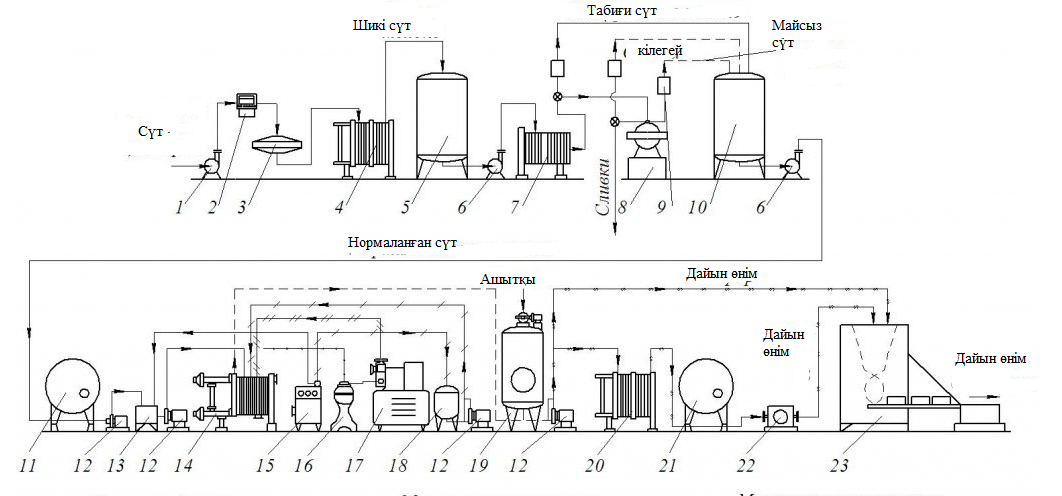
\includegraphics[width=0.9\textwidth]{media/pish2/image24}
	\caption*{1 - сурет. Сүтқышқылды тұздық технологиялық схемасы}
\end{figure}

\begin{multicols}{2}
Антиоксиданттық қасиеттерді жақсарту және дәм сипаттамаларын жақсарту
үшін компонент ретінде аскөк және ақжелкен қолданылды, оның құрамына
күшті антиоксидант -- бетакаротин кіреді, ол біздің денемізді қатерлі
ісіктердің пайда болуынан қорғайды және қартаюды болдырмайды. Ақжелкен
көптеген дәрумендер мен минералдарға бай, мысалы: C, B4, B2, B5 B6, E,
калий, кальций, магний, натрий, фосфор және темір. Осы қасиеттерді
ескере отырып, насыбайгүл атеросклероздың және онымен байланысты
инфаркттардың дамуына жол бермейді, жүрек бұлшықетінің жұмысын
жақсартады, қан тамырларының жалпы жағдайын нығайтады, жүрек құрысуын
азайтады. Бета каротин қандағы холестеринді төмендетеді, бұл
артерияларды нығайтуға және жүрек соғысының алдын алуға мүмкіндік
береді.

Сонымен қатар, өнімді дәрумендер мен минералдармен байыту үшін қияр
таңдалды, олардың құрамында көптеген дәрумендер бар: В\textsubscript{4},
Е, С, РР және минералдар: натрий, калий, кальций, магний, фосфор.
Атеросклероз кезінде РР дәрумені мен талшықтар қандағы холестерин
мөлшерін реттейді, оның артық мөлшерін жеңуге көмектеседі. Жүрек-қан
тамырлары ауруларында, калий мөлшері жоғары, РР дәрумені қан қысымын
төмендетеді, тамыр қабырғаларын нығайтады, жүйке жүйесінің бұзылуларымен
олар церебральды қан айналымын қалыпқа келтіреді және жұмсақ седативті
әсерге ие, орталық жүйке жүйесі мен перифериялық жүйке жүйесі жұмысын
жақсартады. Ас қорыту проблемалары үшін талшық тағамның қорытылуын және
сіңуін жақсартады, асқазан-ішек жолдарының бұзылуына көмектеседі.

Кептірілген сарымсақ дәмдік көрсеткіштерімен сипаттамаларын жақсартумен
қатар, өнімді адам ағзасына жағымды әсер ететін дәрумендер мен
минералдармен байытады. Оның құрамында көптеген дәрумендер бар, олардың
ішінде С, Е, РР және В тобы ерекше назар аударуға лайық, сонымен қатар
генитурарлы жүйенің денсаулығына әсер ететін мырыш сияқты
микроэлементтер адам денсаулығы үшін өте маңызды, денені жасартады және
иммундық жүйені нығайтады.

Сүтқышқылды тұздық технологиясын жасауда өсімдік қоспасы ретінде
аскөктен басқа қияр қосылады. Қиярдың майдалап кесіп тұздық негізіне
қосады. Қиярлардың химиялық құрамын қарастыратын болсақ, оның құрамында:
су (95\%), ақуыз(0,8\%), ауыстырылатын және ауыстырылмайтын амин
қышқылдардың аз мөлшері, жылпы көмірсулар (3\%), крахмал (0, 1\%),
клетчатка (0, 7\%); минералды заттар (мг\%): натрий (8), калий (141),
кальций (28), магний(14), фосфор (42), хлор (25), темір (0, 9), йод,
марганец, мыс, цинк,фтор; витаминдер (мг\%): С (4---18), Е (0, 1), В1,
(0, 03), В2 (0, 04), В6 (0,04), РР (0,2), пантотен қышқылы, аз мөлшерде
бос органикалық қышқылдар, эфир майы, түрлі ферменттер болады.

Дәмдеуіш ретінде аскөк және ақжелкені қолданылады. Өсімдік қоспалары бар
сүтқышқылды тұздық жасау үшін резервуар әдісі таңдалды. Бұл әдіс энергия
шығынын және өндіріс орындарын азайтуға көмектеседі. Резервуарлық
әдіспен өндіріс кезінде ашыту кезінде өнімнің консистенциясы мен
қышқылдығын бақылауға және реттеуге болады. Сүтқышқылды тұздықтарының
ассортиментіне арналған толтырғыштар негізінен табиғи компоненттер болып
табылады.

Сүтқышқылды тұздықтың технологиялық схемасы келесі операциялардан
тұрады: шикізатты қабылдау және сапасын бағалау; шикізат мөлшерін есепке
алу; сүтті тазарту; салқындату; резервирлеу; жылыту; қалыпқа келтіру;
гомогенизация; пастерлеу; салқындату; ашыту; ашыту; араластыру; қоспаны
жасау; салқындату; құю; орау және таңбалау. Өндіріс технологиясының
аяқталу сәті - өнімді көлік контейнерлеріне орау.

Сүтқышқылды тұздық өндіру процесінің технологиялық схемасы 2-суретте
көрсетілген.
\end{multicols}

\begin{figure}[H]
	\centering
	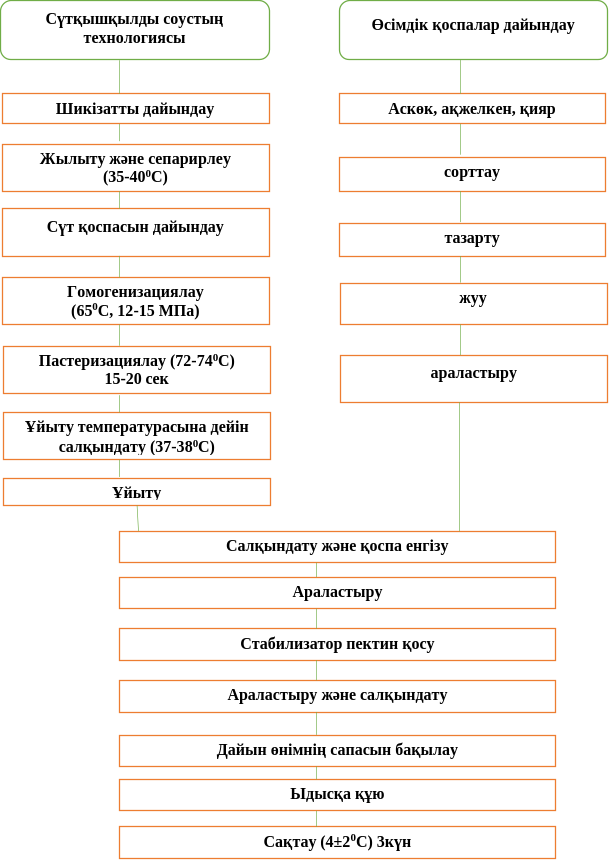
\includegraphics[width=0.55\textwidth]{media/pish2/image25}
	\caption*{2 - сурет. Сүтқышқылды тұздықтың технологиялық схемасы}
\end{figure}

Зерттелінетін сүтқышқылды тұздық үшін энергетикалық құндылығы бойынша
деректер 6-кестеде келтірілген.

\begin{table}[H]
\caption*{6 - кесте. Сүтқышқылды тұздықтың энергетикалық құндылығы}
\centering
\begin{tblr}{
  width = \linewidth,
  colspec = {Q[240]Q[115]Q[98]Q[133]Q[350]},
  cells = {c},
  cell{1}{1} = {r=2}{},
  cell{1}{2} = {c=3}{0.346\linewidth},
  cell{1}{5} = {r=2}{},
  vlines,
  hline{1,3-4} = {-}{},
  hline{2} = {2-4}{},
}
Өнім               & Химиялық құрамы, \% &        &            & Энергетикалық құндылығы, Кдж \\
                   & Ақуыздар            & Майлар & Көмірсулар &                              \\
Сүтқышқылды тұздық & 2,5                 & 1,7    & 2,56       & 155,6                        
\end{tblr}
\end{table}

\begin{multicols}{2}
{\bfseries Қорытынды.} Осылайша эксперименттік және әдеби деректерге
жүргізілген зерттеулер нәтижесінде алғаш рет өсімдіктер қоспасы қосылған
функционалды ашытылған тұздықтар алу мүмкүндігі дәлелденді.

Мақалада тұтас және майсыздандырылған сүттің физика-химиялық
көрсеткіштері талданып, майсыздандырылған сүттегі В дәрумендерінің
мөлшері мен сүтқышқылды өнімдеріндегі маңызды микрофлораның құрамы
анықталды. Зерттеудің келесі кезеңінде таңдалған микроорганизмдердің
сүтқышқылды тұздығын ашыту процесіне әсері зерттеліп, технологиялық
схема ұсынылды. Өнімді резервуарлық әдіспен өндіру барысында аскөк пен
ақжелкен сияқты өсімдік қоспалары дәмдеуіш ретінде қолданылды.

Зерттеу нәтижелері бойынша сүтқышқылды тұздығының энергетикалық
құндылығы мен технологиялық схемасы ұсынылды. Тұздыққа қосылатын өсімдік
шикізатының (аскөк, ақжелкен, қияр, сарымсақ) оңтайлы мөлшері - 3-5\%.
Сондай-ақ, жаңа дайындалған сүтқышқылды тұздығының энергетикалық
құндылығын төмен калориялы өнім ретінде сипаттауға мүмкіндік беретін
көрсеткіштер алынды (ақуыз - 2,7 г, май - 1,7 г, көмірсулар -- 2,56 г).
Құрамында өсімдік қоспалары бар сүтқышқылды тұздығы пайдалы өнім екені
сөзсіз және бірқатар артықшылықтарға ие. Бұл өнім адам ағзасына қажетті
дәрумендер мен минералдарға бай, сонымен қатар ішек микрофлорасын
жақсартуға ықпал етеді. Сондықтан өсімдік қоспалары бар сүтқышқылды
тұздығы салауатты өмір салтын ұстанатын тұтынушылар үшін тиімді таңдау
бола алады.
\end{multicols}

\begin{center}
{\bfseries Әдебиеттер}
\end{center}

\begin{references}
1. Ганина В.И. К вопросу о функциональных продуктах питания / В.И.
Ганина, И.И. Ионова // Молочная промышленность. - 2018. - № 3. --С.
44-46.

2. Рогов И.А., Орешкин Е.Н., Сергеев В.Н. Медико-технологические аспекты
разработки и производства функциональных пищевых продуктов // Пищевая
промышленность. -- 2017. -№ 1. -С. 13--15.

3. Федосова, А. Н. Биотехнология молочных продуктов: учебное пособие для
направления подготовки 19.03.03 -- продукты питания животного
происхождения. профиль -- технология молока и молочных продуктов /
А.Н. Федосова, М.В. Каледина. -Белгород: БелГАУ им.В.Я.Горина, 2019. -
144 с.

4. Қазақстан Республикасының денсаулық сақтау саласын дамытудың 2026
жылға дейінгі тұжырымдамасын бекіту туралы: Қазақстан Республикасы
Үкіметінің 2022 жылғы 24 қарашадағы № 945 қаулысы. URL:
https://adilet.zan.kz/kaz/docs/P2200000945.

5. Диханбаева Ф.Т., Алимарданова М.К., Мухтарханова Р.Б. Сүт саласындағы
өндірістерді жобалау: оқу құралы. -Алматы: Лантар Трейд, 2021. -214 б.
ISBN 978 601-7669-14-0

6. Диханбаева, Ф.Т. Технология молока и производственный учет: учебное
пособие. - Алматы: АТУ, 2015. - 386 с. ISBN 978-601-7166-25-0

7. Диханбаева, Ф. Т. Сүт өнімдерінің технологиясы: оқу құралы. - Алматы:
АТУ, 2014. -167 б. ISBN 978-601-263-253-8

8. Kryuchkova V.V., Gorlov I. F., Belik S.N., Kamlatsky A.S. Vegetable
ingredients in functional fermented milk products // IOP Conference
Series: Earth and Environmental Science. -- 2020. -- Vol. 548:
082092.DOI 10.1088/1755-1315/548/8/082092.

9. Симонова К. М. Разработка технологии соуса кисломолочного: дис.
\ldots{} канд. техн. наук: 05.18.04 / К.М. Симонова. -Омск, 2008. -
199 с.

10. Бредихин С. А. Технология и техника переработки молока: учебное
пособие / С.А. Бредихин. -2-е изд., доп. -М.: Изд-во НИЦ ИНФРА-М,
2021. - 443 с. ISBN 978-5-16-109531-7.

11. Карпеня М.М. Технология производства молока и молочных продуктов:
Учебное пособие / М.М. Карпеня, В.И. Шляхтунов, В.Н. Подрез. -- М.:
Изд-во НИЦ ИНФРА-М, 2015. -- 410 с. ISBN 978-985-475-709-4.

12. Старовойтова К.В., Терещук Л.В., Долголюк И.В., Тарлюн М.А.
Использование вторичного молочного сырья в производстве коктейля //
Молочная промышленность. -2020.- № 8. -С. 61--63. DOI
10.31515/1019-8946-2020-08-61-63.

13. Чураков М. М. Разработка технологии кисломолочного соуса для школьного
питания: дис. \ldots{} канд. техн. наук: 05.18.04 / М.М. Чураков.
--Москва, 2008. --246 с.

14. Тюрина Л.Е., Александрова М.Г., Табаков Н.А. Нетрадиционные молочные и
кисломолочные продукты: учебное пособие / Л.Е. Тюрина, М.Г.
Александрова, Н.А. Табаков. -- Красноярск: Красноярский
государственный аграрный университет, 2010. -- 96 с.

15. Габриелян Д.С., Грунская В.А. Технологические аспекты производства
обогащенных кисломолочных продуктов с использованием молочной
сыворотки // Молочнохозяйственный вестник. -- 2016. -- № 4 (24). --С.
80-91.

16. Росляков Ю.Ф., Шмалько Н.А., Бочкова Л.К. Перспективы использования
амаранта в пищевой индустрии // Известия высших учебных заведений.
Северо-Кавказский регион. Технические науки. -- 2004. -- № 4. -- С.
92--95.

17. Наймушина Е.Г. Теоретическое обоснование и разработка технологии
плодоовощных пектиносодержащих соусов: дис. \ldots{} канд. техн. наук:
05.18.01 / Е.Г. Наймушина. -- Краснодар, 2002. -- 211 с.

18. Волкова Н.Н. Разработка способа получения низкокалорийных эмульсионных
соусов на основе натуральных ингредиентов: дис. \ldots{} канд. техн.
наук: 05.18.06 / Н. Н. Волкова. -- Москва, 2008. -- 127 с.

19. He S., Hekmat S. Sensory Evaluation of Non-Dairy Probiotic Beverages
// Journal of Food Research. --2015. --Vol. 4(1). -P. 186-192. DOI
10.5539/jfr.v4n1p186.

20. ҚР СТ ИСО 707-2011 Сүт және сүт өнімдері. Сынамаларды іріктеу
жөніндегі басшылық. --Астана, 2011.

21. МЕМСТ ҚР СТ 1732-2007 Сүт және сүт өнімдері. Сапа көрсеткіштерін
анықтаудың органолептикалық әдісі. -- Астана, 2007.

22. ГОСТ 5867-90. Молоко и молочные продукты. Методы определения жира. --
Офиц. изд. -- М.: Стандартинформ, 2009. -- Дата введения 01.07.1991.

23. ГОСТ 3624-92. Молоко и молочные продукты. Титриметрические методы
определения кислотности. -- Офиц. изд. -- М.: Стандартинформ, 2009. --
Дата введения 01.01.1994.

24. ГОСТ 34212-2017 Петрушка свежая. Технические условия. -- Введ.
01.07.2018. -- Москва: Стандартинформ, 2017.

25. Жаркова И.М., Мирошниченко Л.А., Звягин А.А., Бавыкина И.А.
Амарантовая мука: характеристика, сравнительный анализ, возможности
применения // Вопросы питания. -- 2014. --Т. 83. -№ 1. -С. 67-73.
\end{references}

\begin{center}
{\bfseries References}
\end{center}

\begin{references}
1. Ganina V.I. K voprosu o funkcional' nyh produktah
pitanija / V.I. Ganina, I.I. Ionova // Molochnaja
promyshlennost'. - 2018. - № 3. --S. 44-46. {[}in
Russian{]}

2. Rogov I.A., Oreshkin E.N., Sergeev V.N. Mediko-tehnologicheskie
aspekty razrabotki i proizvodstva funkcional' nyh
pishhevyh produktov // Pishhevaja promyshlennost'. --
2017. -№ 1. -S. 13--15. {[}in Russian{]}

3. Fedosova, A. N. Biotehnologija molochnyh produktov: uchebnoe posobie
dlja napravlenija podgotovki 19.03.03 -- produkty pitanija zhivotnogo
proishozhdenija. profil'{} -- tehnologija moloka i
molochnyh \\produktov / A.N. Fedosova, M.V. Kaledina. -Belgorod: BelGAU
im.V.Ja.Gorina, 2019. - 144 s. {[}in Russian{]}

4. Qazaqstan Respýblıkasynyń densaýlyq saqtaý salasyn damytýdyń 2026
jylǵa deıingi tujyrymdamasyn bekitý týraly: Qazaqstan Respýblıkasy
Úkimetiniń 2022 jylǵy 24 qarashadaǵy № 945 qaýlysy. URL:\\
\href{https://adilet.zan.kz/kaz/docs/P2200000945}{https://adilet.zan.kz}. {[}in Kazakh{]}

5. Dıhanbaeva F.T., Alımardanova M.K., Mýhtarhanova R.B. Sút salasyndaǵy
óndiristerdi jobalaý: oqý quraly. -Almaty: Lantar Treıd, 2021. -214 b.
ISBN 978 601-7669-14-0 {[}in Kazakh{]}

6. Dihanbaeva, F.T. Tehnologija moloka i proizvodstvennyj uchet: uchebnoe
posobie. - Almaty: ATU, 2015. - 386 s. ISBN 978-601-7166-25-0 {[}in
Russian{]}

7. Dıhanbaeva, F. T. Sút ónimderiniń tehnologıasy: oqý quraly. - Almaty:
ATÝ, 2014. -167 b. ISBN 978-601-263-253-8 {[}in Kazakh{]}

8. Kryuchkova V.V., Gorlov I. F., Belik S.N., Kamlatsky A.S. Vegetable
ingredients in functional \\fermented milk products // IOP Conference
Series: Earth and Environmental Science. -- 2020. -- Vol. 548:
082092. DOI 10.1088/1755-1315/548/8/082092.

9. Simonova K. M. Razrabotka tehnologii sousa kislomolochnogo: dis.
\ldots{} kand. tehn. nauk: 05.18.04 / K.M. Simonova. -- Omsk, 2008. --
199 s. {[}in Russian{]}

10. Bredihin S. A. Tehnologija i tehnika pererabotki moloka: uchebnoe
posobie / S.A. Bredihin. -- 2-e izd., dop. -- M.: Izd-vo NIC INFRA-M,
2021. -- 443 s. ISBN 978-5-16-109531-7. {[}in Russian{]}

11. Karpenja M.M. Tehnologija proizvodstva moloka i molochnyh produktov:
Uchebnoe posobie / M.M. Karpenja, V.I. Shljahtunov, V.N. Podrez. -- M.:
Izd-vo NIC INFRA-M, 2015. -- 410 s. ISBN 978-985-475-709-4. {[}in
Russian{]}

12. Starovojtova K.V., Tereshhuk L.V., Dolgoljuk I.V., Tarljun M.A.
Ispol' zovanie vtorichnogo \\molochnogo
syr' ja v proizvodstve koktejlja // Molochnaja
promyshlennost'. -2020.- № 8. -S. 61--63. DOI
10. 31515/1019-8946-2020-08-61-63. {[}in Russian{]}

13. Churakov M. M. Razrabotka tehnologii kislomolochnogo sousa dlja
shkol' nogo pitanija: dis. \ldots{} kand. tehn. nauk:
05. 18.04 / M.M. Churakov. --Moskva, 2008. --246 s. {[}in Russian{]}

14. Tjurina L.E., Aleksandrova M.G., Tabakov N.A. Netradicionnye
molochnye i kislomolochnye produkty: uchebnoe posobie / L.E. Tjurina,
M.G. Aleksandrova, N.A. Tabakov. -- Krasnojarsk: Krasnojarskij\\
gosudarstvennyj agrarnyj universitet, 2010. -- 96 s. {[}in Russian{]}

15. Gabrieljan D.S., Grunskaja V.A. Tehnologicheskie aspekty proizvodstva
obogashhennyh \\kislomolochnyh produktov s ispol' zovaniem
molochnoj syvorotki // Molochnohozjajstvennyj vestnik. -- 2016. -- № 4
(24). --S. 80-91. {[}in Russian{]}

16. Rosljakov Ju.F., Shmal' ko N.A., Bochkova L.K.
Perspektivy ispol' zovanija amaranta v pishhevoj
industrii // Izvestija vysshih uchebnyh zavedenij. Severo-Kavkazskij
region. Tehnicheskie nauki. -- 2004. -- № 4. -- S. 92--95. {[}in
Russian{]}

17. Najmushina E.G. Teoreticheskoe obosnovanie i razrabotka tehnologii
plodoovoshhnyh \\pektinosoderzhashhih sousov: dis. \ldots{} kand. tehn.
nauk: 05.18.01 / E.G. Najmushina. -- Krasnodar, 2002. -- 211 s. {[}in
Russian{]}

18. Volkova N.N. Razrabotka sposoba poluchenija nizkokalorijnyh
jemul' sionnyh sousov na osnove\\
natural' nyh ingredientov: dis. \ldots{} kand. tehn.
nauk: 05.18.06 / N. N. Volkova. -- Moskva, 2008. -- 127 s. {[}in
Russian{]}

19. He S., Hekmat S. Sensory Evaluation of Non-Dairy Probiotic Beverages
// Journal of Food Research. --2015. --Vol. 4(1). -P. 186-192. DOI
10. 5539/jfr.v4n1p186.

20. QR ST ISO 707-2011 Sút jáne sút ónimderi. Synamalardy irikteý
jónindegi basshylyq. --Astana, 2011. {[}in Kazakh{]}

21. MEMST QR ST 1732-2007 Sút jáne sút ónimderi. Sapa kórsetkishterin
anyqtaýdyń organoleptıkalyq ádisi. - Astana, 2007. {[}in Kazakh{]}

22. GOST 5867-90. Moloko i molochnye produkty. Metody opredelenija zhira.
-- Ofic. izd. -- M.: \\Standartinform, 2009. -- Data vvedenija 01.07.1991.
{[}in Russian{]}

23. GOST 3624-92. Moloko i molochnye produkty. Titrimetricheskie metody
opredelenija kislotnosti. -- Ofic. izd. -- M.: Standartinform, 2009. --
Data vvedenija 01.01.1994. {[}in Russian{]}

24. GOST 34212-2017 Petrushka svezhaja. Tehnicheskie uslovija. -- Vved.
01. 07.2018. -- Moskva: \\Standartinform, 2017. {[}in Russian{]}

25. Zharkova I.M., Miroshnichenko L.A., Zvjagin A.A., Bavykina I.A.
Amarantovaja muka: harakteristika, sravnitel' nyj analiz,
vozmozhnosti primenenija // Voprosy pitanija. -- 2014. --T. 83. -№ 1.
-S. 67-73. {[}in Russian{]}
\end{references}

\begin{authorinfo}
\emph{{\bfseries Авторлар туралы мәліметтер}}

Есиркеп Г.Е.-техника ғылымдарың кандидаты, қауымдастырылған профессор,
Қ.Құлажанов атындағы Қазақ технология және бизнес университеті, Астана,
Қазақстан,e-mail: milana.anar@mail.ru;

Диханбаева Ф.Т.- техника ғылымдарының докторы, Алматы технологиялық
университеті, Алматы, Қазақстан, e-mail: fatima6363@mail.ru;

Шунекеева А.А. -PhD, профессорлар ассистенті, Ш. Уалиханов атындағы
Көкшетау университеті, Көкшетау, Қазақстан, e-mail:
alma-shunekeeva@mail.ru;

Ботбаева Ж.Т.- биология ғылымдарының кандадаты, Қ.Құлажанов атындағы
Қазақ технология және бизнес университеті, Астана, Қазақстан,
e-mail.zhanar.b.t@mail.ru;

Нармандах Ж.- магистр, ассистент, Қ. Құлажанов атындағы Қазақ технология
және бизнес университеті, Астана, Қазақстан, e-mail:
zhupar10\_89@mail.ru.

\emph{{\bfseries Information about the authors}}

Esirkep G.E. - Candidate of Technical Sciences, Associate Professor,
Kazakh University of Technology and Business named after K. Kulazhonov,
Astana, Kazakhstan, e-mail: milana.anar@mail.ru;

Dikhanbaeva F.T. - Doctor of Technical Sciences, Almaty Technology
University, Almaty, Kazakhstan, e-mail: \\fatima6363@mail.ru;

Shunekeeva Alma Aitkozhaevna -- PhD, assistant professors, Kokshetau
University named after Sh. Ualikhanov, Kokshetau, Kazakhstan, e-mail:
alma-shunekeeva@mail.ru;

Botbayeva Zhanar Turlybekovna -- candidate of Biological Sciences,
Kazakh University of Technology and Business named after K. Kulazhonov,
Astana, Kazakhstan. e-mail: zhanar.b.t@mail.ru;

Narmandakh Zh. - Master's Degree, Assistant, Kazakh University of
Technology and Business named after K. Kulazhonov, Astana, Kazakhstan,
e-mail: zhupar10\_89@mail.ru.
\end{authorinfo}
